\documentclass[a4paper, 12pt]{article}
\usepackage[T2A]{fontenc}
\usepackage[utf8]{inputenc}
\usepackage[english,russian]{babel}
\usepackage{amsmath, amsfonts, amssymb, amsthm, mathtools, misccorr, indentfirst, multirow}
\usepackage{wrapfig}
\usepackage{graphicx}
\usepackage{subfig}
\usepackage{adjustbox}
\usepackage{pgfplots}

\usepackage{siunitx}

\usepackage{geometry}
\geometry{top=20mm}
\geometry{bottom=20mm}
\geometry{left=20mm}
\geometry{right=20mm}
\newcommand{\angstrom}{\textup{\AA}}
\begin{document}
\begin{titlepage}
    \newpage
    \begin{center}
     Министерство науки и высшего образования Российской федерации \\ ФЕДЕРАЛЬНОЕ ГОСУДАРСТВЕННОЕ АВТОНОМНОЕ \\ ОБРАЗОВАТЕЛЬНОЕ УЧРЕЖДЕНИЕ ВЫСШЕГО ОБРАЗОВАНИЯ \\ «МОСКОВСКИЙ ФИЗИКО-ТЕХНИЧЕСКИЙ ИНСТИТУТ \\ (НАЦИОНАЛЬНЫЙ ИССЛЕДОВАТЕЛЬСКИЙ УНИВЕРСИТЕТ)» \\ (МФТИ, Физтех)
    \end{center}
    
    \vspace{15em}
    
    \begin{center}
    КАФЕДРА ТВЕРДОТЕЛЬНОЙ ЭЛЕКТРОНИКИ \\
    \vspace{1em}
    ОТЧЕТ\\
    ПО ЛАБОРАТОРНОЙ РАБОТЕ \\
    \vspace{1em}
    ИЗУЧЕНИЕ ХАРАКТЕРИОГРАФА И МЕТОДОВ ВИЗУАЛЬНОГО НАБЛЮДЕНИЯ СТАТИЧЕСКИХ ХАРАКТЕРИСТИК ПОЛУПРОВОДНИКОВЫХ ДИОДОВ
    \end{center}

    \vspace{10em}
    \begin{flushleft}
        Работу выполнили \hspace{17em} \underline{\hspace{3cm}}
        И.Д. Бессонов \\
         \hspace{26em} \underline{\hspace{3cm}} Е.С. Иванова \\
          \hspace{26em} \underline{\hspace{2.6cm}} Е.О. Коробкина\\
        \hspace{26em}
        \raisebox{-\baselineskip}{\shortstack{\underline{\hspace{3cm}}\\(подпись, дата)}}     
        И.С. Потапова
    \end{flushleft}

    \vspace{1em}

    \begin{flushleft}
        Работу принял, оценка
        \hspace{15em}
        \raisebox{-\baselineskip}{\shortstack{\underline{\hspace{5cm}}\\(подпись, дата, оценка)}}
    \end{flushleft}

    \vspace{5em}
    
    \begin{center}
        Долгопрудный, 2025
    \end{center}
\end{titlepage}

\newpage
\tableofcontents

\newpage
\section{Аннотация}
\textbf{Цель работы:}
Ознакомиться с принципом работы характериографа, измерить ВАХ двух полупроводниковых образцов.
    
   
\section{Ход работы}
 В данной работе было предложено снять ВАХ для двух устройств: германиевого диода Д310 и кремниевого стабилитрона Д814A.\\

 Как видно из характеристик, диод Д310 имеет напряжение пропускания 0,15 В в прямом направлении, в обратном направлении пробой диода происходит при 50 В, таким образом он выполняет основную функцию диода - пропускать ток только в одном направлении.

Стабилитрон же в свою очередь имеет напряжение пропускания около 0,5 В, напряжение стабилизации при этом - 7.5 В.

На основе полученных ВАХ и по предположению о том, что они следуют закону вида 
\begin{equation}
    \label{main}
    \centering
    I_\text{д} = I_{d_0} (e^{\frac{V}{\theta \varphi_T}} - 1),
\end{equation}
 где $\varphi_T$ - температурный потенциал при комнатной температуре равный 26 мВ, далее будут вычислены параметры $I_{d_0}$ (диффузионный ток) и $\theta$ (коэффициент неидеальности) для имеющихся образцов (см. задание 5). 

 У идеального диода $\theta=1$, поэтому формула принемает вид: 
 \begin{equation}
    \label{main}
    \centering
    I_\text{д} = I_{d_0} (e^{\frac{V}{\varphi_T}} - 1).
\end{equation}


\subsection{Практическая часть}
\begin{figure}[h]
    \centering
    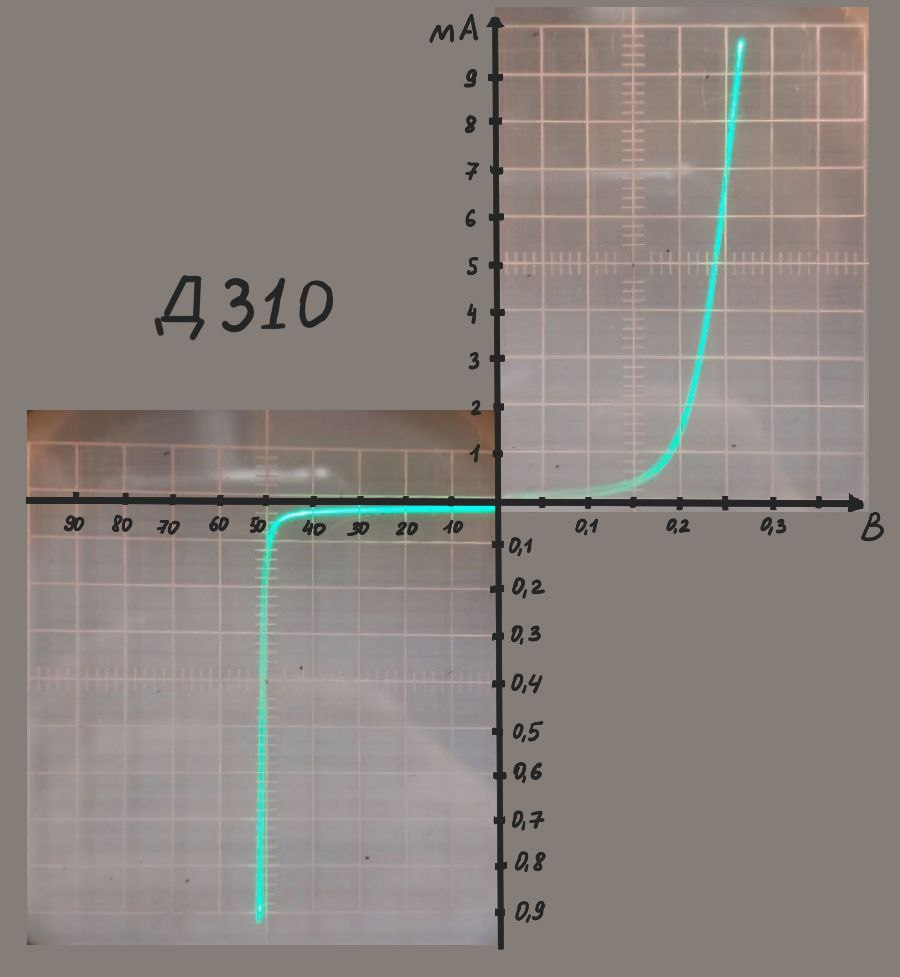
\includegraphics[width = 0.4\linewidth]{img/D310.jpg}
    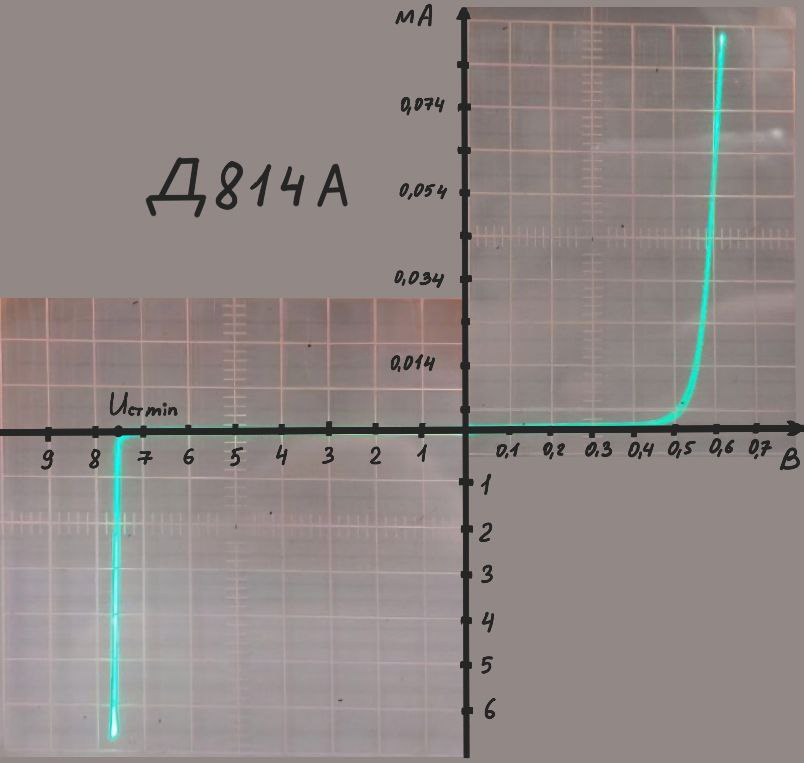
\includegraphics[width = 0.46\linewidth]{img/D814.jpg}
    \caption{ВАХ полупроводникового диода и стабилитрона, полученные на характериографе.}
\end{figure}

\newpage
\subsection{Теоретическая часть}

Построим графики ВАХ для идеального диода по формуле (2) и сравним теоретические кривые с полученными экспереминтальными точками.
\begin{figure}[h!]
    \centering
    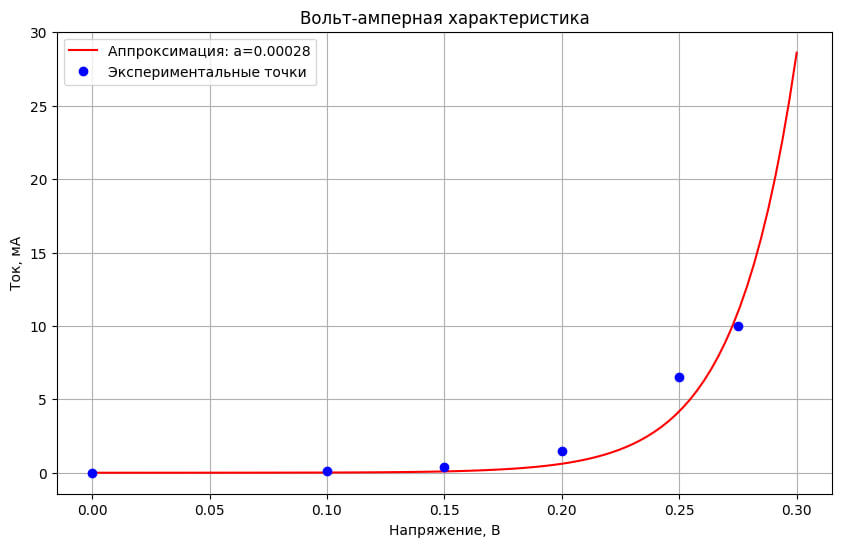
\includegraphics[width =0.92 \linewidth]{img/photo_5287677535850720017_y.jpg}
    \caption{ВАХ идеального диода и экспериментальные точки полупроводникового диода}
\end{figure}
\begin{figure}[h!]
    \centering
    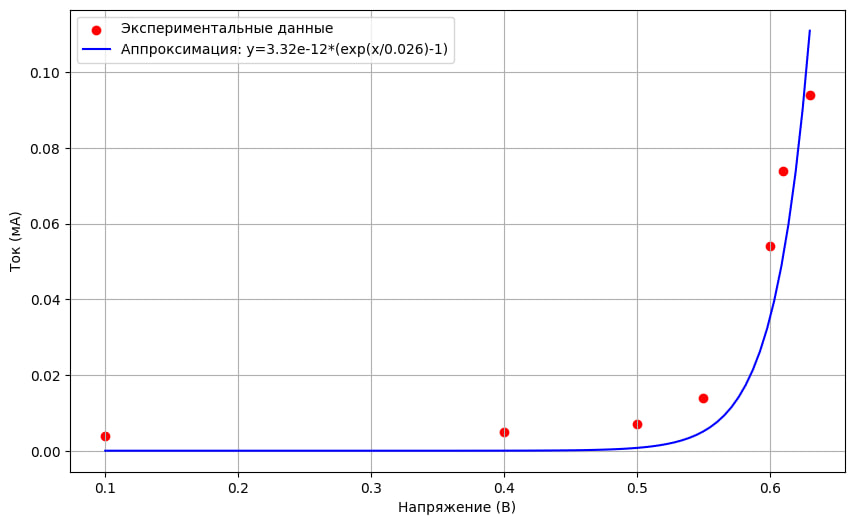
\includegraphics[width =0.92 \linewidth]{img/photo_5289929335664405770_y.jpg}
    \caption{ВАХ идеального диода и экспериментальные точки стабилитрона}
\end{figure}

Диффузионный ток или обратный ток насыщения, полученный при апроксимации в случае полупроводникового диода равен 0,28 мкА, а в случае стабилитрона: $3,32 \cdot 10^{-9}$ мкА.

Сравним экспериментальные ВАХ с ВАХами диодов: Д310 и Д814А. Соответсвующие напряжения для используемых диодов представлены в таблице, данные взяты с сайтов производителей данных типов диодов: 

\begin{table}[h]
\centering
\begin{tabular}{|c|c|c|}
\hline
Образец & $U_{\text{пропускания}}$, B  & $U_{\text{пробоя}}$, B  \\ \hline
Д310    & 0,1 - 0,2 & 20 \\ \hline
Д814А    & 0,5 - 1 & 7,0 - 8,5 \\ \hline
\end{tabular}
\end{table}

Видим, что полученные нами экспериментальные напряжения диодов сходятся с найденными выше.

Для диода Д310 найдена соответствующая ему ВАХ, которая хорошо сходится с полученной в ходе эксперимента:  

\begin{figure}[!h]
    \centering
    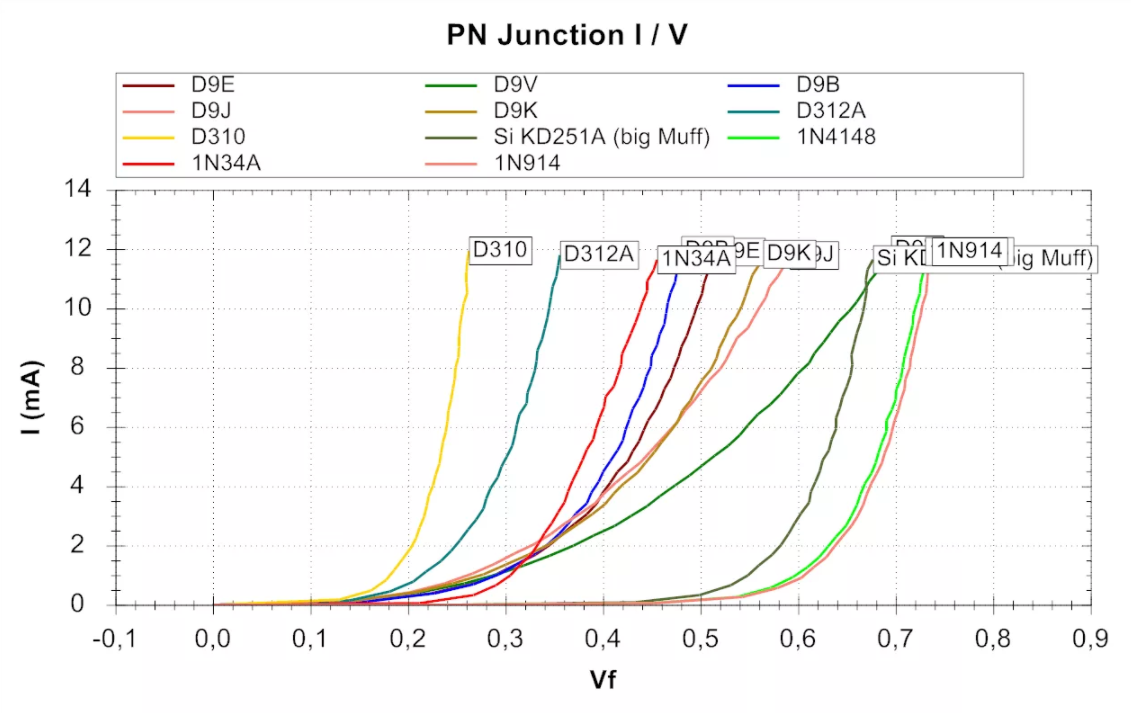
\includegraphics[width = 0.95\linewidth]{img/theor.png}
    \caption{ВАХ Д310}
\end{figure}


\newpage

\subsection{Задание 5}
Считая, что ВАХ описывается формулой (1), найдем коэффициенты неидеальности и диффузионный ток для полупроводникового диода и стабилитрона:

\begin{figure}[h]
    \centering
    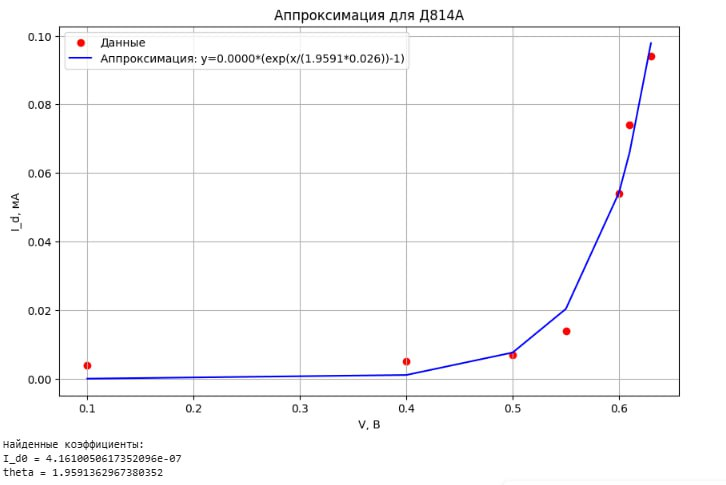
\includegraphics[width =0.72 \linewidth]{img/photo_2025-02-12_03-14-46.jpg}
    \caption{Аппроксимация для полупроводникового диода}

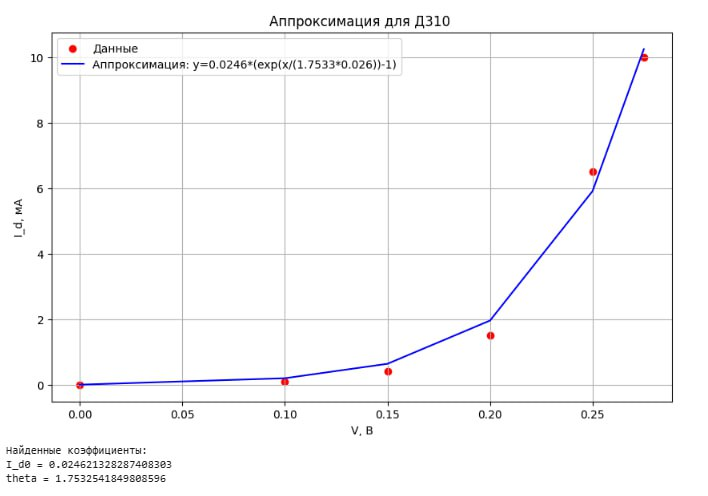
\includegraphics[width =0.72 \linewidth]{img/photo_2025-02-12_03-14-48.jpg}
    \caption{Аппроксимация для полупроводникового диода и стабилитрона}
\end{figure}



\section{Выводы}
В ходе лабораторной работы мы получили вольт-амперные характеристики полупроводниковых приборов, а так же научились пользоваться характериографом. 

С помощью графиков зависимости тока $I_\text{д}$ от напряжения $V$ рассчитали обратный ток насыщения $I_{d_0}$ для случая идеального диода, а также для неидеального, определили коэффициент неидельности $\theta$:

\begin{table}[h]
\centering
\begin{tabular}{|c|c|c|}
\hline
Образец & Д310   & Д814А \\ \hline
$I_{d_0}$, мкА & 0,28 & 3.32$\cdot 10^{-9}$ \\ \hline
\end{tabular}
\caption{Данные для идеального диода}
\end{table}

\begin{table}[h]
\centering
\begin{tabular}{|c|c|c|}
\hline
Образец & $I_{d_0}$, мА  & $\theta$ \\ \hline
Д310    & 4,2$\cdot 10^{-7}$ & 1,96 \\ \hline
Д814А    & 0,025 & 1,75 \\ \hline
\end{tabular}
\caption{Данные для неидеального диода}
\end{table}
Сравнили полученные экспериментально характеристики с данными, указанными на сайте производителя, получили, что результаты сходятся.

\section{Список литературы}
\begin{itemize}
    \item \textbf{Лабораторная работа №16 }: Изучение характериографа и методов визуального наблюдения и измерения статических характеристик полупроводниковых приборов/МФТИ. - М., 1987. - 47 с.
    \item  https://provodpro.ru/content/voltage-drop-of-germanium-diode-k.html
\end{itemize}





\end{document}

